
\documentclass[english]{article}
\usepackage[T1]{fontenc}
\usepackage[latin9]{inputenc}
\usepackage{geometry}
%\geometry{verbose,tmargin=3cm,bmargin=3cm,lmargin=2cm,rmargin=2cm}
\usepackage{amsmath}
\usepackage{amssymb}
\usepackage{caption}
\usepackage{subcaption}
\usepackage{float}
\usepackage{cancel}
\usepackage{empheq}
\usepackage{tcolorbox}

\newcommand*\widefbox[1]{\fbox{\hspace{2em}#1\hspace{2em}}}

\makeatletter
%%%%%%%%%%%%%%%%%%%%%%%%%%%%%% User specified LaTeX commands.
\usepackage{tikz}
\usepackage{tkz-euclide}
\usetikzlibrary{patterns}
\usetikzlibrary{arrows.meta}

\makeatother

\usepackage{babel}
\begin{document}
\title{Incompressible Flow Solver}
\author{Alberto Padovan}
\maketitle


\section{Cartesian Mesh and Governing Equations}
In this section, we will derive the discretized operators for a 2D problem flow configuration over a cartesian mesh (shown in figure \ref{fig:grid}).
The equations will be spatially discretized using finite volumes on a fully staggered grid to ensure primary conservation and to avoid pressure checkerboarding. 

\begin{figure}[H]
\centering
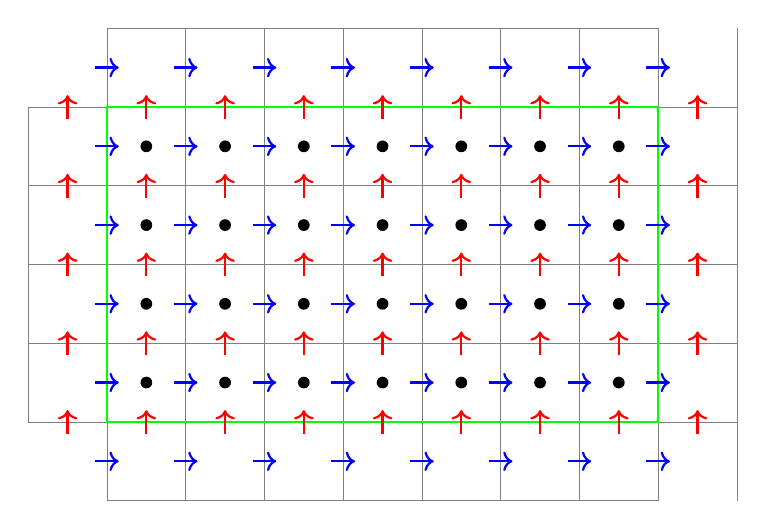
\begin{tikzpicture}
% Create grid and remove corner cells
\draw[step=1cm,color=gray,very thin] (-2,-2) grid (7,4);
\fill[white!40!white, draw = white] (-2,-2) rectangle (-1,-1);
\fill[white!40!white, draw = white] (6,-2) rectangle (7,-1);
\fill[white!40!white, draw = white] (-2,3) rectangle (-1,4);
\fill[white!40!white, draw = white] (6,3) rectangle (7,4);
\draw[step=1cm,color=gray,very thin] (-2,1) grid (-1,3);
\draw[step=1cm,color=gray,very thin] (-1,1.5) grid (-0.5,4);
\draw[step=1cm,color=gray,very thin] (6,1.5) grid (6,4);
\draw[step=1cm,color=gray,very thin] (6,2) grid (7,3);
\draw[step=1cm,color=gray,very thin] (5,-2) grid (6,-1);
\draw[step=1cm,color=gray,very thin] (6,-1) grid (7,0);
\draw[step=1cm,color=gray,very thin] (-1,-2) grid (0,-1);
\draw[step=1cm,color=gray,very thin] (-2,-1) grid (-1,0);

\draw[step=1cm,color=green,thick] (-1,-1) rectangle (6,3);

\foreach \i in {-1.5,-0.5,0.5,...,6.5}{
  \foreach \j in {-1,0,...,3}{
    \draw[->,red,thick] (\i,\j-0.15)--(\i,\j+0.15);
  }
}


\foreach \i in {-1,0,...,6}{
  \foreach \j in {-1.5,-0.5,0.5,...,3.5}{
    \draw[->,blue,thick] (\i-0.15,\j)--(\i+0.15,\j);
  }
}

\foreach \i in {-0.5,0.5,...,5.5}{
  \foreach \j in {-0.5,0.5,...,2.5}{
    \node at (\i,\j) [circle,fill,inner sep=1.5pt]{};
  }
}


% \foreach \x in {-2,-1,0,1,2,3,4,5,6,7}
%     \node[below] at (\x,-2.1) {\small \x};
%   \foreach \y in {-2,-1,0,1,2,3,4}
%   \node[left] at (-2.1,\y) {\small \y};
  
\end{tikzpicture}
\caption{Staggered grid. The green line denotes the boundaries of the physical domain. Velocity and pressure values \emph{inside} the blue domain are active degrees of freedom that must be solved for. Velocities \emph{on} or \emph{outside} the blue lines are boundary/ghost points that can be determined algebraically given the boundary conditions and the interior values. Blue arrows indicate $x$-velocities, red arrows $y$-velocities, and black dots denote pressure.}
\label{fig:grid}
\end{figure}

\noindent Before proceeding we recall the conservative form of the incompressible Navier-Stokes along with continuity.

\begin{align}
\partial_t \mathbf{u} + \nabla \cdot \left(\mathbf{u}\mathbf{u}^\top \right) &=  - \nabla p + Re^{-1}\nabla^2 \mathbf{u} \\
\nabla \cdot \mathbf{u} &= 0
\end{align}
\noindent The integral form of the eqautions is obtained by integrating over the volume. The divergence theorem is used to turn the volume integrals into surface integrals, where $\mathbf{\hat{n}}$ denotes the outward-pointing, unit-norm vector normal to the surface. (In our 2D setting over a cartesian grid, we have $\mathbf{\hat{n}} = (1,0)$ or $\mathbf{\hat{n}} = (0,1)$.)

\begin{align}
  \label{eq:ns_equation}
  \int _{\mathcal{V}} \partial_t \mathbf{u}\, \mathrm{d}\mathcal{V} + \int_{\mathcal{S}} \mathbf{u}\left(\mathbf{u}\cdot \mathbf{\hat{n}}\right)\,\mathrm{d}\mathcal{S} &=  - \int _{\mathcal{S}} p\mathbf{\hat{n}}\, \mathrm{d}\mathcal{S} + Re^{-1}\int_{\mathcal{S}} \mathbf{\hat{n}} \cdot \nabla \mathbf{u} \,\mathrm{d}\mathcal{S} \\
  \label{eq:cont_equation}
\int_{\mathcal{S}} \mathbf{u} \cdot \mathbf{\hat{n}}\,\mathrm{d}\mathcal{S} &= 0.
\end{align}


\subsection{$x$-momentum equation in conservative form}

\begin{figure}[H]
\centering
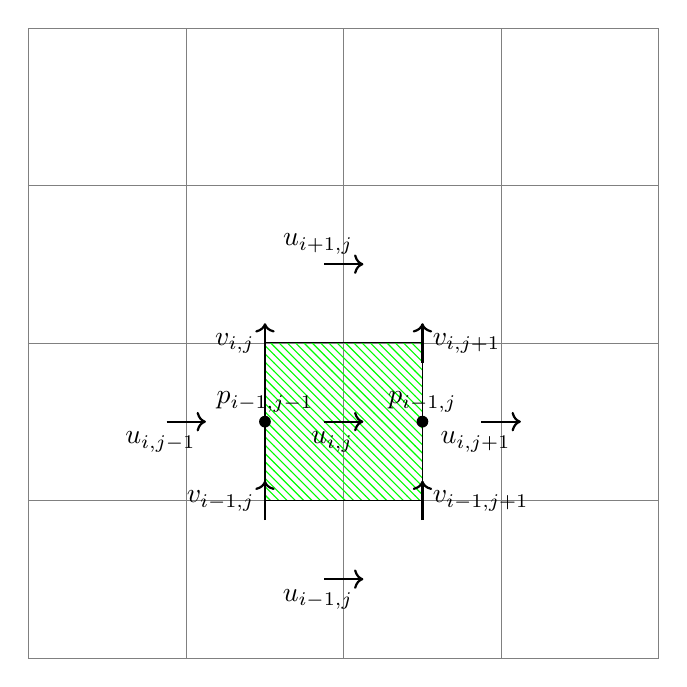
\begin{tikzpicture}
% Create grid and remove corner cells
\draw[step=2cm,color=gray,very thin] (-4.01,-4.01) grid (4,4);
\draw[pattern=north west lines, pattern color=green] (-1,-2) rectangle (1,0);

% u velocities
\draw[thick,->] (-0.25,-1) -- (0.25,-1) node[anchor=north east] {$u_{i,j}$};
\draw[thick,->] (1.75,-1) -- (2.25,-1) node[anchor=north east] {$u_{i,j+1}$};
\draw[thick,->] (-2.25,-1) -- (-1.75,-1) node[anchor=north east] {$u_{i,j-1}$};
\draw[thick,->] (-0.25,1) -- (0.25,1) node[anchor=south east] {$u_{i+1,j}$};
\draw[thick,->] (-0.25,-3) -- (0.25,-3) node[anchor=north east] {$u_{i-1,j}$};

% v velocities
\draw[thick,->] (-1,-0.25) -- (-1,0.25) node[anchor=north east] {$v_{i,j}$};
\draw[thick,->] (1,-0.25) -- (1,0.25) node[anchor=north west] {$v_{i,j+1}$};
\draw[thick,->] (1,-2.25) -- (1,-1.75) node[anchor=north west] {$v_{i-1,j+1}$};
\draw[thick,->] (-1,-2.25) -- (-1,-1.75) node[anchor=north east] {$v_{i-1,j}$};

\node at (-1,-1) [circle,fill,inner sep=1.5pt]{};
\tkzDefPoint(-1,-1){A}
\tkzLabelPoint[above](A){$p_{i-1,j-1}$}

\node at (1,-1) [circle,fill,inner sep=1.5pt]{};
\tkzDefPoint(1,-1){B}
\tkzLabelPoint[above](B){$p_{i-1,j}$}


\end{tikzpicture}
\caption{Control volume for $x$-momentum. The grid spacing in the $x$ direction is $\Delta x$, and $\Delta y$ in the $y$ direction.}
\label{fig:grid_x}
\end{figure}

Starting from equation \eqref{eq:ns_equation} in the $x$ direction, we have
\begin{equation}
  \int _{\mathcal{V}} \partial_t u\, \mathrm{d}\mathcal{V} + \int_{\mathcal{Y}} u^2\,\mathrm{d}\mathcal{Y} +\int_{\mathcal{X}} uv\,\mathrm{d}\mathcal{X}  =  - \int _{\mathcal{Y}} p\, \mathrm{d}\mathcal{Y} + Re^{-1}\left(\int_{\mathcal{Y}} \partial_x u\,\mathrm{d}\mathcal{Y} + \int_{\mathcal{X}} \partial_y u\,\mathrm{d}\mathcal{X}\right).
\end{equation}
In discrete form, using the control volume in figure \ref{fig:grid_x}, we have
\begin{equation}
  \begin{aligned}
    \int _{\mathcal{V}} \partial_t u\, \mathrm{d}\mathcal{V} &= \partial_t u_{i,j}\Delta x \Delta y\\
    \int_{\mathcal{Y}} u^2\,\mathrm{d}\mathcal{Y} &= \frac{\Delta y}{4}\left(\left(u_{i,j+1} + u_{i,j}\right)^2 - \left(u_{i,j+1} + u_{i,j}\right)^2\right) \\
    \int_{\mathcal{X}} uv\,\mathrm{d}\mathcal{X} &= \frac{\Delta x}{4}\left(\left(u_{i+1,j} + u_{i,j}\right)\left(v_{i,j} + v_{i,j+1}\right) - \left(u_{i-1,j} + u_{i,j}\right)\left(v_{i-1,j} + v_{i-1,j+1}\right)\right)\\
    \int _{\mathcal{Y}} p\, \mathrm{d}\mathcal{Y} &= \left(p_{i-1,j} - p_{i-1,j-1}\right)\Delta y \\
    Re^{-1}\int_{\mathcal{Y}} \partial_x u\,\mathrm{d}\mathcal{Y} &= \frac{Re^{-1}}{\Delta x}\left(u_{i,j+1} - 2 u_{i,j} + u_{i,j-1}\right)\Delta y \\
    Re^{-1}\int_{\mathcal{X}} \partial_y u\,\mathrm{d}\mathcal{X} &= \frac{Re^{-1}}{\Delta y}\left(u_{i+1,j} - 2 u_{i,j} + u_{i-1,j}\right)\Delta x
  \end{aligned}
\end{equation}
Putting this all together and dividing through by $\Delta x \Delta y$, we obtain

\begin{empheq}[box=\widefbox]{align*}
  &\partial_t u_{i,j} + \frac{1}{4\Delta x}\left(\left(u_{i,j+1} + u_{i,j}\right)^2 - \left(u_{i,j+1} + u_{i,j}\right)^2\right) \\
  &+ \frac{1}{4\Delta y}\left(\left(u_{i+1,j} + u_{i,j}\right)\left(v_{i,j} + v_{i,j+1}\right) - \left(u_{i-1,j} + u_{i,j}\right)\left(v_{i-1,j} + v_{i-1,j+1}\right)\right)\\
  &= -\frac{p_{i-1,j} - p_{i-1,j-1}}{\Delta x} + Re^{-1}\left(\frac{u_{i,j+1} - 2 u_{i,j} + u_{i,j-1}}{\Delta x^2} + \frac{u_{i+1,j} - 2 u_{i,j} + u_{i-1,j}}{\Delta y^2}\right).
\end{empheq}


\subsection{$y$-momentum equation in conservative form}

\begin{figure}[H]
\centering
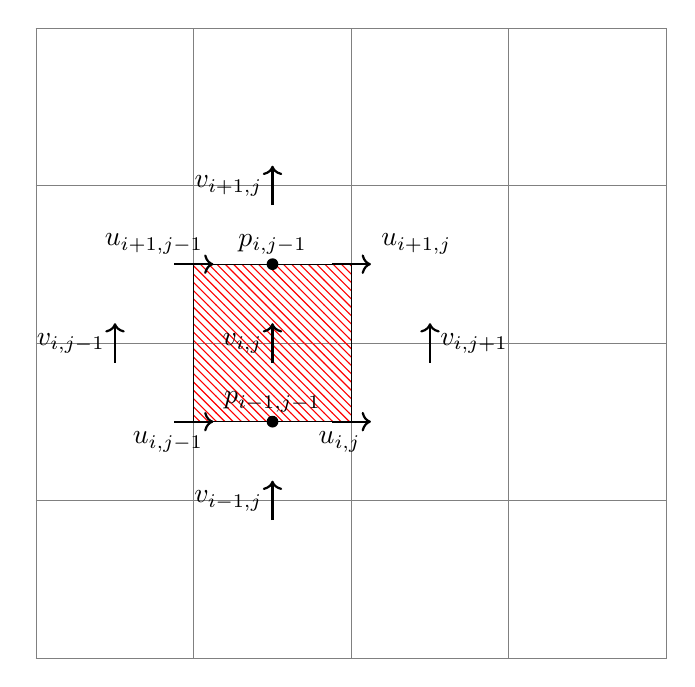
\begin{tikzpicture}
% Create grid and remove corner cells
\draw[step=2cm,color=gray,very thin] (-4.01,-4.01) grid (4,4);
\draw[pattern=north west lines, pattern color=red] (-2,-1) rectangle (0,1);

% u velocities
\draw[thick,->] (-0.25,-1) -- (0.25,-1) node[anchor=north east] {$u_{i,j}$};
\draw[thick,->] (-2.25,-1) -- (-1.75,-1) node[anchor=north east] {$u_{i,j-1}$};
\draw[thick,->] (-0.25,1) -- (0.25,1) node[anchor=south west] {$u_{i+1,j}$};
\draw[thick,->] (-2.25,1) -- (-1.75,1) node[anchor=south east] {$u_{i+1,j-1}$};

% v velocities
\draw[thick,->] (-1,-0.25) -- (-1,0.25) node[anchor=north east] {$v_{i,j}$};
\draw[thick,->] (1,-0.25) -- (1,0.25) node[anchor=north west] {$v_{i,j+1}$};
\draw[thick,->] (-3,-0.25) -- (-3,0.25) node[anchor=north east] {$v_{i,j-1}$};
\draw[thick,->] (-1,-2.25) -- (-1,-1.75) node[anchor=north east] {$v_{i-1,j}$};
\draw[thick,->] (-1,1.75) -- (-1,2.25) node[anchor=north east] {$v_{i+1,j}$};


\node at (-1,-1) [circle,fill,inner sep=1.5pt]{};
\tkzDefPoint(-1,-1){A}
\tkzLabelPoint[above](A){$p_{i-1,j-1}$}

\node at (-1,1) [circle,fill,inner sep=1.5pt]{};
\tkzDefPoint(-1,1){B}
\tkzLabelPoint[above](B){$p_{i,j-1}$}


\end{tikzpicture}
\caption{Control volume for $y$-momentum}
\label{fig:grid_y}
\end{figure}


\textcolor{red}{Adi, please derive the y momentum equation like I derived the x momentum equation in the previous subsection.}

\subsection{Continuity equation}
\begin{figure}[H]
\centering
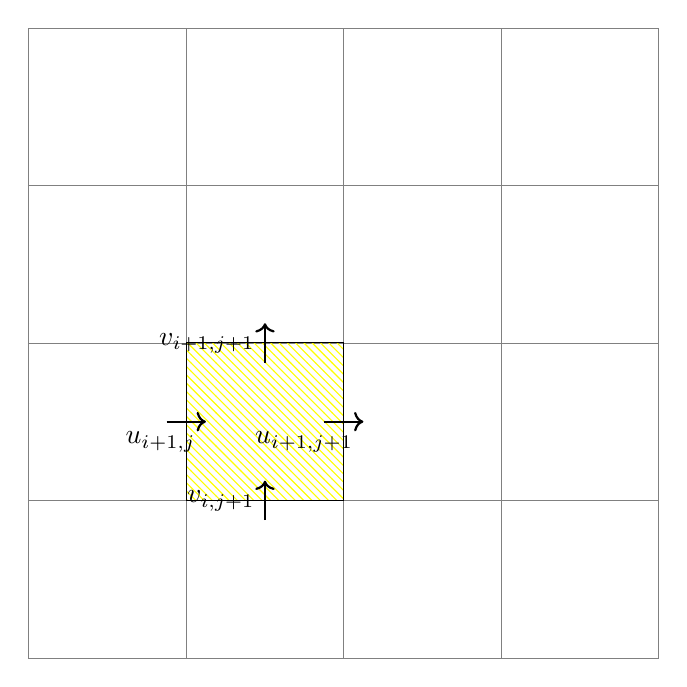
\begin{tikzpicture}
% Create grid and remove corner cells
\draw[step=2cm,color=gray,very thin] (-4.01,-4.01) grid (4,4);
\draw[pattern=north west lines, pattern color=yellow] (-2,-2) rectangle (0,0);

% u velocities
\draw[thick,->] (-0.25,-1) -- (0.25,-1) node[anchor=north east] {$u_{i+1,j+1} $};
\draw[thick,->] (-2.25,-1) -- (-1.75,-1) node[anchor=north east] {$u_{i+1,j}$};

% v velocities
\draw[thick,->] (-1,-0.25) -- (-1,0.25) node[anchor=north east] {$v_{i+1,j+1}$};
\draw[thick,->] (-1,-2.25) -- (-1,-1.75) node[anchor=north east] {$v_{i,j+1}$};
\end{tikzpicture}
\caption{Control volume for the continuity equation.}
\label{fig:contGrid}
\end{figure}
Starting from equation \eqref{eq:cont_equation}, and using the control volume in figure \ref{fig:contGrid}, we have
\begin{equation}
  \left(u_{i+1,j+1} - u_{i+1,j}\right)\Delta y + \left(v_{i+1,j+1} - v_{i,j+1}\right)\Delta x = 0.
\end{equation}
Dividing through by $\Delta x$ and $\Delta y$, we obtain
\begin{equation*}
  \boxed{\frac{1}{\Delta x}\left(u_{i+1,j+1} - u_{i+1,j}\right) + \frac{1}{\Delta y}\left(v_{i+1,j+1} - v_{i,j+1}\right) = 0.}
\end{equation*}


\end{document}

%%% Local Variables:
%%% mode: LaTeX
%%% TeX-master: t
%%% End:
